\section{Study }

\subsection{Jorge Cham's Dissertation - openloop control of 1DOF vertical hopper }
\begin{figure}[h]
\centering

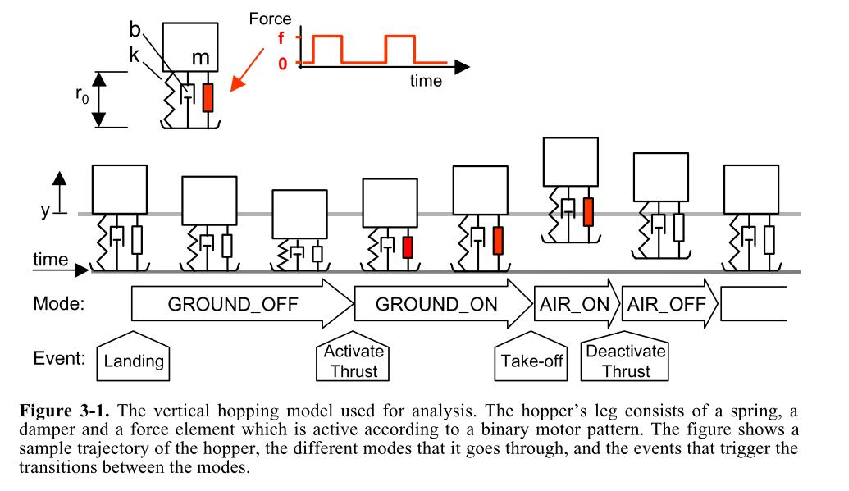
\includegraphics{test.pdf} 
\caption{The schematic of a 1 DOF hopper \cite{Cham2002}}
\label{fig.1DOF-Hopper}
\end{figure}

\subsubsection{System assumptions}
\begin{itemize}
\item massless leg
\item open-loop force control
\end{itemize}
\subsubsection{Sequence}
\{AIR\_OFF, GROUND\_OFF, GROUND\_ON, AIR\_ON\}


\subsubsection{Equation of motion}
Using the model as shown in Fig. \ref{fig.1DOF-Hopper}, during the stand phase (i.e. $y\leq 0$), the equation of motion can be expressed as:
\begin{align*}
m \ddot y = -b\dot y +-ky -mg + f
\end{align*}
\noindent where $m$ is the mass, $b$ is the damping, $k$ is the stiffness, $f$ is the control input.
Normalized by weight, the equation becomes
\begin{align*}
 \ddot y = -b/m\dot y +-k/my -g + f/m
\end{align*}

\noindent Expressed in state space form:

\begin{align}
\begin{bmatrix}
\dot y  \\
\ddot y 
\end{bmatrix} = \begin{bmatrix}
0 & 1 \\
-k/m & -b/m
\end{bmatrix}\begin{bmatrix}
 y  \\
\dot y 
\end{bmatrix} + 
\begin{bmatrix}
0  \\
-g+f/m 
\end{bmatrix}
\end{align}
or equivalently
\begin{align}
\label{eq:groundEOM}
\dot X = \begin{bmatrix}
0 & 1 \\
-\omega^2 & -2\xi\omega
\end{bmatrix}X + 
\begin{bmatrix}
0  \\
-g+f_n(t)
\end{bmatrix} &= AX+B
\end{align}
where $X \triangleq [y,\dot y]^T$.
When the hopper is in the air (i.e. $y> 0$, flight phase), 
\begin{align}
\label{eq:airEOM}
\dot X = \begin{bmatrix}
0 & 1 \\
0 & 0
\end{bmatrix}X + 
\begin{bmatrix}
0  \\
-g 
\end{bmatrix}
\end{align}
\noindent Define the force  of an open-loop motor pattern
\begin{align}
 f_n(t)=\begin{cases}
    f/m, & \text{if $t_{off}<t<t_{off}+t_{on}$}.\\
    0, & \text{otherwise}.
  \end{cases}
\end{align}

\noindent\textbf{Solutions}

For \eqref{eq:airEOM}:
\begin{align}
\label{eq:airEOMsol}
X(t) = \begin{bmatrix}
1 & t \\
0 & 0
\end{bmatrix}X_0 + 
\begin{bmatrix}
t^2/2  \\
 t
\end{bmatrix}(-g)
\end{align}

For \eqref{eq:groundEOM} when actuator is on:
\begin{align}
\label{eq:groundEOMsol}
X(t) = e^{At}(X_0-X_{eq_{on}}) + X_{eq_{on}}
\end{align}

For \eqref{eq:groundEOM} when actuator is off:
\begin{align}
\label{eq:groundEOMsol2}
X(t) = e^{At}(X_0-X_{eq_{off}}) + X_{eq_{off}}
\end{align}

where $X_{eq_{on}}$ and $X_{eq_{off}}$ are the equilibrium states:
\begin{align}
\label{eq:eqStates}
X_{eq_{on}} &= [\frac{f_n-g}{\omega^2}, 0]^T\\
X_{eq_{off}}&= [\frac{-g}{\omega^2}, 0]^T
\end{align}

\subsubsection{Stability Analysis}
\textbf{Eigen values}
For \eqref{eq:airEOM}, eigen values are $\pm 1$, in inherently unstable. (Why this does not matter? Because the contact)

\noindent For \eqref{eq:groundEOM}, eigen values are
$-\xi\omega \pm \omega\sqrt{(\xi^2-1)} = -\omega(\xi \pm \sqrt{\xi^2 -1}) = -\omega(\xi \pm i\sqrt{1-\xi^2 })$ As long as \omega  and \xi are larger than zero, the system is stable.\\

\pagebreak

\noindent\textbf{Poincare Method: The rest part skipped}\\
Reasons: For more complex systems, hard to analytically derive the Poincare map (usually no closed-form solution). Found a package in spokeRunner simulation for Poincare Analysis (numerically), plan to reuse it.

\begin{figure}[H]
\centering

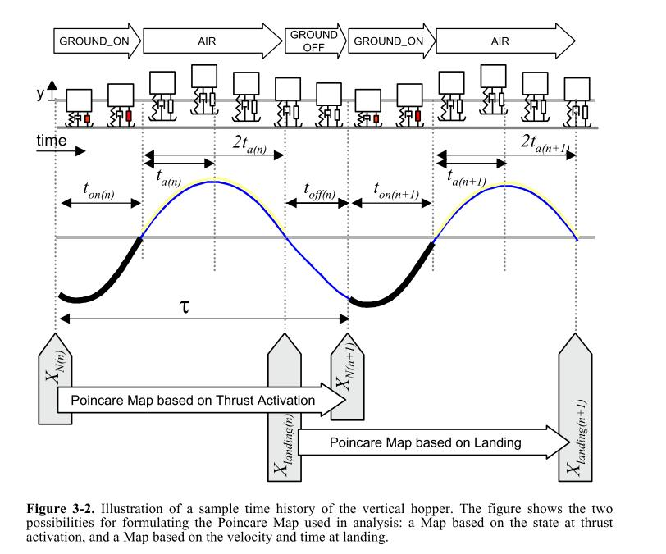
\includegraphics{modes.pdf} 
\caption{The modes of the hopper \cite{Cham2002}}
\label{fig.modes}
\end{figure}

Assumptions:
\begin{itemize}
\item the period is T
\item two modes need to be checked
\item $X(0) = X_{N_n}$ where $n$ indicates the $n^{th}$ trajectory
\end{itemize}

\noindent Using Equations \ref{eq:groundEOMsol}, we can derive
\begin{align*}
X(t_{on_n} )= e^{At_{on_n}}(X_{N_n} - X_{eq_{on}})+ X_{eq_{on}}
\end{align*}
\noindent Use the fact that 
\begin{align*}
X(t_{on_n}+2t_{a_n}) = -X(t_{on_n} ) 
\end{align*}

\noindent Then we can calculate the $X_{N_{n+1}}$ as follows:
\begin{align}
\nonumber X_{N_{n+1}} &= e^{A(T-2t_{a_n}-t_{on_n})}(-X(t_{on_n} ) - X_{eq_{off}}) + X_{eq_{off}}\\\
\nonumber X_{N_{n+1}} &= e^{A(T-2t_{a_n}-t_{on_n})}(-e^{At_{on_n}}(X_{N_n} - X_{eq_{on}})- X_{eq_{on}} ) - X_{eq_{off}}) + X_{eq_{off}}\\
&= X_{eq_{off}}-e^{A(T-2t_{a_n})}(X_{N_n}-X_{e_{on}}) -e^{A(T-2t_{a_n}-t_{on_n})}( X_{eq_{on}}+ X_{eq_{off}})
\end{align}

About the second switch surface $X_{landing_n}$,
\begin{align}
X_{landing_n} = -X(t_{on_n} ) =- e^{At_{on_n}}(X_{N_n} - X_{eq_{on}})- X_{eq_{on}}
\end{align}

\pagebreak
\subsection{Jerry's proof for pitch stability }

\pagebreak